\documentclass{ctexart}
\usepackage{amsmath, mathrsfs, amsfonts}
\usepackage{tikz}
\usepackage{graphicx}
% library



\begin{document}
    
\begin{figure}[htp]    % 输入bfi,按回车会自动出现整个figure的片段
    \centering
    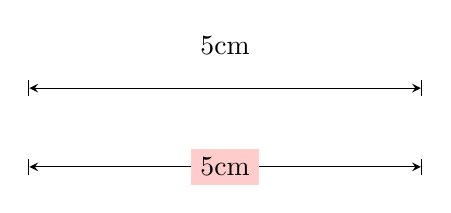
\begin{tikzpicture}[>=stealth]
        \draw[|<->|] (0,0)--node[above=3mm]{5cm}(5,0);    % node 结点 above below right left % 在tikz中所有的命令均要以分号来结尾,和c语言、c#、c++类似
        \draw[|<->|] (0,-1)--node[fill=red!20!white]{5cm}(5,-1);    % 填充 20%red 80%white



        % \draw[|<->|] (0,-1) to (5,-1);
        % \draw[dashed] (0,-2) to (5,-2);
        % \draw[dotted] (0,-3) to (5,-3);
        % \draw[dashdotted] (0,-4) to (5,-4);
        % \draw[|<->|,dashed] (0,-5) to (5,-5);    % 选项的顺序不会有任何影响
        % \draw[|<->|,dashed,thick] (0,-6) to (5,-6);
        % \draw[|<->|,dashed,very thick] (0,-7) to (5,-7);
        % \draw[|<->|,dashed,ultra thick] (0,-8) to (5,-8);
        % \draw[|<->|,thin] (0,-9) to (5,-9);






    \end{tikzpicture}
    \caption{}
\end{figure}

\begin{figure}[htp]
    \centering
    \begin{tikzpicture}[>=latex]
        \draw[->] (-1,0)--(4,0)node[right]{$x$};
        \draw[->] (0,-1)--(0,4)node[right]{$y$};
        % \draw (0,2)node[left]{$N$}--(2,2)node[right]{$P(x,y)$}--(2,0)node[below]{$M$};
        \node at (-.2,-.2){$O$};

        % \draw (0,1)node[left]{$1$}--(.1,1);
        % \draw (0,2)node[left]{$2$}--(.1,2);
        % \draw (0,3)node[left]{$3$}--(.1,3);
        % \draw (1,0)node[below]{$1$}--(1,.1);
        
        \foreach \x in {1,2,...,6}
        {
            \draw (0,\x*0.5)node[left]{$\x$}--(.1,\x*0.5);
            \draw (\x*0.5,0)node[below]{$\x$}--(\x*0.5,.1);
        }



    \end{tikzpicture}

    \caption{<caption>}
\end{figure}












\end{document}